% ============================================================================
% ARTIGO DO PROJETO DE APLICACAO | APRENDIZADO DE MAQUINA PARA SAUDE - UFF
% Projeto editavel no Overleaf: pdfLaTeX + BibTeX; citacoes ABNT autor-data.
% Secoes em arquivos separados (secoes/*.tex) para reaproveitar o texto na
% versao SBCAS. Numeros conferidos contra resultados/*.csv do repositorio.
% ============================================================================
\documentclass[11pt,a4paper]{article}

% Idioma, caracteres e tipografia
\usepackage[T1]{fontenc}
\usepackage[utf8]{inputenc}
\usepackage[brazil]{babel}
\usepackage{lmodern}
\usepackage{microtype}
\usepackage{setspace}

% Pagina, estrutura e estilo
\usepackage[a4paper,top=2.55cm,bottom=2.5cm,left=2.75cm,right=2.65cm]{geometry}
\usepackage{xcolor}
\usepackage{titlesec}
\usepackage{fancyhdr}
\usepackage{graphicx}
\usepackage{booktabs}
\usepackage{adjustbox}
\usepackage{tabularx}
\usepackage{array}
\usepackage{caption}
\usepackage{amsmath}
\usepackage{tikz}
\usetikzlibrary{positioning,arrows.meta}
\usepackage{enumitem}
\PassOptionsToPackage{hyphens}{url}
\usepackage[colorlinks=true,linkcolor=black,citecolor=azulescuro,urlcolor=azulescuro]{hyperref}
\usepackage[alf]{abntex2cite}
\urlstyle{same}

\definecolor{azulescuro}{RGB}{22,62,83}
\definecolor{cinzasec}{RGB}{96,107,115}
\definecolor{linha}{RGB}{213,221,224}
\definecolor{azulclaro}{RGB}{241,246,247}

\setstretch{1.12}
\setlength{\parindent}{1.25em}
\setlength{\parskip}{0.21em}
\setlength{\emergencystretch}{2em}
\captionsetup{font=small,labelfont=bf,justification=centering}
\titleformat{\section}{\large\sffamily\bfseries\color{azulescuro}}{\thesection}{0.70em}{}
\titleformat{\subsection}{\normalsize\sffamily\bfseries\color{azulescuro}}{\thesubsection}{0.65em}{}
\titlespacing*{\section}{0pt}{1.4em}{0.55em}
\titlespacing*{\subsection}{0pt}{1.05em}{0.35em}
\renewcommand{\refname}{Referências}
\addto\captionsbrazil{\renewcommand{\tablename}{Tabela}}
\setlength{\headheight}{14pt}
\pagestyle{fancy}
\fancyhf{}
\fancyhead[L]{\footnotesize\sffamily\color{cinzasec} APRENDIZADO DE MÁQUINA PARA SAÚDE}
\fancyhead[R]{\footnotesize\sffamily\color{cinzasec} UFF}
\fancyfoot[C]{\footnotesize\color{cinzasec}\thepage}
\renewcommand{\headrulewidth}{0.3pt}
\renewcommand{\footrulewidth}{0pt}
\fancypagestyle{plain}{\fancyhf{}\fancyfoot[C]{\footnotesize\color{cinzasec}\thepage}\renewcommand{\headrulewidth}{0pt}}

\begin{document}

% =========================== TITULO E AUTORES ================================
\begin{center}
  {\sffamily\footnotesize\color{azulescuro}\bfseries PROJETO DE APLICAÇÃO \enspace|\enspace ARTIGO CIENTÍFICO}\par
  \vspace{0.65em}
  {\LARGE\sffamily\bfseries Aprendizado de Máquina versus Escore de Mayo: qual vale mais a pena na predição de óbito em cirrose biliar primária?}\par
  \vspace{0.8em}
  {\normalsize Clayton Escouper das Chagas}\par
  \vspace{0.15em}
  {\small Instituto de Computação -- Universidade Federal Fluminense}\par
  {\small\color{cinzasec} Aprendizado de Máquina para Saúde \enspace|\enspace 2026.2}\par
  \vspace{0.85em}
  {\color{linha}\rule{\linewidth}{0.8pt}}
\end{center}
\vspace{-0.7em}

% ================================ RESUMO =====================================
\begin{center}
\textbf{\sffamily Resumo}
\end{center}
\vspace{-0.85em}
\begin{quote}
\small
O Escore de Risco de Mayo, um modelo de Cox com cinco variáveis de rotina publicado em 1989, ainda é a referência clássica para estimar o prognóstico na cirrose biliar primária, hoje chamada colangite biliar primária. Este estudo mede o valor incremental do aprendizado de máquina sobre uma regressão logística com as mesmas cinco variáveis na predição de óbito em até cinco anos, usando os 312 pacientes rotulados do conjunto público da Mayo Clinic (UCI 878), dos quais 115 morreram no horizonte. O desenho 2 x 2 cruza a família de métodos (regressão e aprendizado de máquina, com \textit{random forest} e XGBoost) e o conjunto de variáveis (5 e 17), com validação cruzada estratificada repetida 5 x 5, ajuste de hiperparâmetros aninhado, validação quase externa nos pacientes não randomizados e um braço de controle de vazamento. A regressão com cinco variáveis obteve AUROC média de 0,906 e inclinação de calibração de 1,04. Nenhum modelo de aprendizado de máquina mostrou ganho: as diferenças de AUROC em relação à referência ficaram entre $-$0,013 e 0,000, todas com intervalos de Bonferroni que incluem zero, e a maior diferença nominal foi a da regressão penalizada com 17 variáveis (+0,009). Usar o tempo de seguimento como entrada, como na competição Kaggle Playground S3E26, reduziu o \textit{log loss} de 0,753 para 0,645 com uma informação indisponível no momento da predição. Neste estudo de caso, o aprendizado de máquina não justificou sua complexidade adicional diante de um modelo de regressão de cinco variáveis.
\end{quote}
\vspace{-0.35em}
\noindent\textbf{Palavras-chave:} colangite biliar primária; escore de Mayo; aprendizado de máquina; valor incremental; calibração; vazamento de dados.
\vspace{0.55em}

% =============================== INTRODUCAO ==================================
% Sem subsecoes: contexto -> problema -> lacuna -> pergunta/objetivo -> contribuicoes.
\section{Introdução}\label{sec:introducao}

A cirrose biliar primária (CBP) é uma doença hepática crônica e autoimune que destrói progressivamente os pequenos ductos biliares do fígado e pode evoluir para cirrose, insuficiência hepática e necessidade de transplante. Como a maioria dos pacientes não tem cirrose no diagnóstico, a doença passou a ser chamada, a partir de 2015, de colangite biliar primária, mantendo a sigla \cite{beuers2015nomenclature}. Este artigo usa o nome antigo porque é o que consta no conjunto de dados e na literatura que o originou. A evolução da doença varia muito entre pacientes, e estimar o risco individual de óbito na primeira avaliação ajuda a definir a intensidade do acompanhamento e o momento de encaminhamento ao transplante.

Desde 1989 existe uma ferramenta para essa estimativa: o Escore de Risco de Mayo, um modelo de regressão de Cox com cinco variáveis de rotina (idade, bilirrubina, albumina, tempo de protrombina e edema), derivado de um ensaio clínico conduzido na Mayo Clinic entre 1974 e 1984 \cite{dickson1989prognosis}. Os dados desse ensaio são públicos e se tornaram um conjunto clássico de ensino e de teste de métodos, primeiro em análise de sobrevivência \cite{fleming1991counting} e, depois, em aprendizado de máquina (AM), inclusive no repositório da UCI \cite{uci878} e na competição Kaggle Playground S3E26 \cite{reade2023ps3e26}. Modelos de AM prometem mais precisão, mas costumam trazer custos: perdem a transparência de uma fórmula que o médico calcula à beira do leito, exigem mais infraestrutura e, quando usam variáveis além das cinco de Mayo, exigem também mais exames e mais pacientes com dados completos.

A pergunta relevante para a prática, portanto, não é se um modelo de AM é preciso, mas se ele é \textbf{mais} preciso que a ferramenta já disponível, e a que custo. Esse é o conceito de valor incremental: o benefício adicional que um novo modelo traz em comparação com o método clínico em uso. Uma revisão sistemática de 71 estudos não encontrou vantagem do AM sobre a regressão logística quando a comparação tinha baixo risco de viés, e observou que 79\% dos estudos não avaliaram calibração \cite{christodoulou2019systematic}. No conjunto da Mayo Clinic, o problema é agravado pelo enquadramento mais difundido da tarefa: a competição do Kaggle pede a classificação do desfecho em três classes usando o tempo de seguimento como variável de entrada, uma informação que só existe depois do desfecho e que caracteriza vazamento de dados \cite{kapoor2023leakage}.

Este trabalho pergunta quanto o AM acrescenta a um modelo de regressão com as cinco variáveis do Escore de Mayo na predição de óbito em até cinco anos, e se um eventual ganho viria do algoritmo ou das variáveis extras. O objetivo é medir esse valor incremental em discriminação e calibração, num desenho 2 x 2 que cruza a família de métodos (regressão e AM) e o conjunto de variáveis (as 5 de Mayo e as 17 do conjunto de dados), avaliado nos mesmos pacientes e nas mesmas partições.

As contribuições são quatro: (i) uma comparação controlada entre regressão e AM em que todos os modelos usam as mesmas partições, o mesmo orçamento de ajuste e transformações aprendidas só no treino; (ii) a quantificação do valor incremental com intervalos de confiança pareados e correção para comparações múltiplas, acompanhada da avaliação de calibração; (iii) a medida de quanto o enquadramento com vazamento infla o desempenho; e (iv) código e resultados abertos, com reprodução verificada, seguindo as recomendações do TRIPOD+AI \cite{collins2024tripodai}.

O restante do artigo está organizado da seguinte forma: a Seção~\ref{sec:relacionados} apresenta os trabalhos relacionados; a Seção~\ref{sec:metodos} descreve dados e procedimentos; a Seção~\ref{sec:resultados} apresenta os resultados; a Seção~\ref{sec:discussao} discute implicações e limitações; e a Seção~\ref{sec:conclusao} sintetiza as conclusões.

% =========================== TRABALHOS RELACIONADOS ===========================
\section{Trabalhos relacionados}\label{sec:relacionados}

\subsection{Levantamento e seleção da literatura}
O levantamento foi uma revisão narrativa, sem protocolo sistemático. Foram consultados o PubMed, o Google Acadêmico e repositórios institucionais com combinações de termos sobre a doença (\textit{primary biliary cirrhosis}, \textit{primary biliary cholangitis}, \textit{PBC}) e sobre a tarefa (\textit{prognostic score}, \textit{machine learning}, \textit{survival prediction}), além de buscas pelo próprio conjunto de dados (\textit{UCI cirrhosis patient survival prediction}, \textit{Kaggle playground cirrhosis}). Foram selecionados estudos de três grupos: escores prognósticos derivados por regressão, aplicações de AM em CBP e trabalhos de AM sobre o conjunto da Mayo Clinic. Somaram-se estudos metodológicos sobre comparação entre AM e regressão, calibração e vazamento.

\subsection{Abordagens existentes e comparação crítica}
Os escores clínicos para CBP são, em sua maioria, modelos de regressão de Cox. O Escore de Mayo foi estimado em 312 pacientes dos ensaios randomizados e reestimado com os 418 pacientes da coorte \cite{dickson1989prognosis}. Depois da adoção do ácido ursodesoxicólico como tratamento padrão, surgiram escores para pacientes tratados. O GLOBE foi derivado em 4.119 pacientes de oito países e obteve estatística C de 0,82 na validação \cite{lammers2015globe}. Os escores UK-PBC foram derivados em 1.916 pacientes e validados em 1.249, com áreas sob a curva acima de 0,90 em 5, 10 e 15 anos \cite{carbone2016ukpbc}. Ambos usam variáveis medidas após um ano de tratamento, o que os torna incompatíveis com uma predição feita na linha de base.

Em CBP, o AM aparece sobretudo como ferramenta de descoberta. \citeonline{gerussi2022ml} aplicaram agrupamento não supervisionado a 11.819 pacientes e identificaram quatro perfis com prognósticos distintos, mas não compararam o desempenho preditivo com o de um escore de regressão. No conjunto da Mayo Clinic, os 312 pacientes randomizados serviram como um dos exemplos de \textit{random survival forests} \cite{ishwaran2008rsf}, numa comparação de métodos de sobrevivência que não tinha como foco o valor incremental sobre o Escore de Mayo.

Os trabalhos mais recentes sobre esse conjunto seguem o enquadramento da competição do Kaggle, cujos dados são sintéticos, gerados a partir do conjunto original \cite{reade2023ps3e26}. \citeonline{shakir2025cirrhosis} classificaram o desfecho em três classes, removendo o tempo de seguimento das entradas, e relataram acurácia de 89,55\% com XGBoost após balanceamento sintético de classes. No fluxograma do estudo, o balanceamento aparece antes da divisão entre treino e teste, e não há avaliação de calibração. \citeonline{tu2025cirrhosis} treinou cinco modelos nos dados sintéticos e os testou nos 418 pacientes originais, dos quais os dados sintéticos foram derivados. Ele agrupou censura e transplante como sobrevida, sem horizonte temporal, e relatou acurácia de 89\% com \textit{random forest} e AUC de 0,95 com XGBoost, também sem calibração. A Tabela~\ref{tab:literatura} resume esses estudos.

\begin{table}[htbp]
\centering
\caption{Síntese dos estudos relacionados.}
\label{tab:literatura}
\small
\renewcommand{\arraystretch}{1.14}
\begin{tabularx}{\linewidth}{@{}p{2.55cm}X X X@{}}
\toprule
\textbf{Estudo} & \textbf{Dados e população} & \textbf{Modelagem e avaliação} & \textbf{Limitação central para esta pergunta} \\
\midrule
\citeonline{dickson1989prognosis} & Ensaios da Mayo Clinic; 312 randomizados e 418 no total & Cox com 5 variáveis; validação em coorte independente & Coeficientes estimados nos mesmos dados usados aqui \\
\citeonline{lammers2015globe} & 4.119 pacientes tratados, 8 países & Cox (GLOBE); C de 0,82 na validação & Variáveis após 1 ano de tratamento \\
\citeonline{carbone2016ukpbc} & 1.916 + 1.249 pacientes tratados, Reino Unido & Cox (UK-PBC); AUC acima de 0,90 & Variáveis após 1 ano de tratamento \\
\citeonline{gerussi2022ml} & 11.819 + 1.069 pacientes, internacional & Agrupamento não supervisionado & Sem comparação preditiva com escore \\
\citeonline{ishwaran2008rsf} & 312 randomizados da Mayo Clinic, entre outros & \textit{Random survival forests} & Foco no método, não no valor incremental \\
\citeonline{shakir2025cirrhosis} & Dados sintéticos do Kaggle & 5 classificadores, 3 classes; acurácia & Balanceamento antes da divisão; sem calibração \\
\citeonline{tu2025cirrhosis} & Sintéticos (treino) e 418 originais (teste) & 5 classificadores, binário sem horizonte & Teste nos dados que geraram o treino; sem calibração \\
\bottomrule
\end{tabularx}
\par\vspace{3pt}{\footnotesize\color{cinzasec}Fonte: elaboração própria a partir dos estudos citados.}
\end{table}

No plano metodológico, \citeonline{christodoulou2019systematic} compararam 282 pares de modelos em 71 estudos: nas comparações com baixo risco de viés, a diferença no logito da AUC entre AM e regressão logística foi de 0,00 (IC 95\% de $-$0,18 a 0,18), enquanto nas de alto risco de viés o AM pareceu superior. \citeonline{vancalster2019calibration} chamam a calibração de calcanhar de Aquiles da análise preditiva, porque um modelo pode discriminar bem e ainda assim fornecer probabilidades erradas. \citeonline{kapoor2023leakage} mostram que o vazamento de dados, inclusive o uso de variáveis que não estariam disponíveis no momento da predição, é uma causa frequente de resultados irreprodutíveis em ciência baseada em AM.

\subsection{Lacuna de pesquisa e posicionamento da proposta}
No levantamento realizado, não foi encontrado estudo que compare, nos mesmos dados e nas mesmas partições, modelos de AM com um modelo de regressão com as variáveis do Escore de Mayo, avaliando discriminação e calibração e medindo o efeito do vazamento pelo tempo de seguimento. Este trabalho não propõe um novo modelo nem um novo escore. Ele reproduz, com protocolo controlado, a comparação entre AM e regressão num caso clássico, nos termos sugeridos por \citeonline{christodoulou2019systematic} e \citeonline{steyerberg2014seven}, e quantifica o quanto o enquadramento mais difundido do conjunto infla o desempenho.

% ============================= MATERIAIS E METODOS ============================
\section{Materiais e métodos}\label{sec:metodos}

\subsection{Desenho do estudo e definição da tarefa}
O estudo é uma comparação retrospectiva de modelos de predição clínica, relatada segundo o TRIPOD+AI \cite{collins2024tripodai}. A unidade de análise é o paciente, com uma linha por pessoa e todas as variáveis medidas na data de registro no estudo (linha de base). A tarefa é a classificação binária de óbito em até cinco anos (1.826 dias). O rótulo foi definido assim: pacientes que morreram até 1.826 dias recebem 1; pacientes acompanhados por mais de 1.826 dias, vivos ou mortos depois disso, recebem 0; pacientes censurados ou transplantados antes de 1.826 dias são excluídos, porque não se sabe se teriam morrido no horizonte. Classificar com horizonte fixo, em vez de modelar o tempo até o evento, permite comparar diretamente modelos de classificação e o escore de Cox na mesma métrica, ao custo de excluir esses pacientes.

O desenho é 2 x 2: duas famílias de métodos (regressão e AM), cada uma com as 5 variáveis do Escore de Mayo e com as 17 variáveis do conjunto, nos mesmos pacientes e nas mesmas partições. A leitura horizontal (mesma família) mostra o efeito das variáveis extras. A leitura vertical (mesmas variáveis) compara pipelines, que diferem no algoritmo e também no tratamento dos dados; uma análise de sensibilidade aproxima a comparação do efeito do algoritmo ao dar às árvores o pré-processamento da regressão.

\subsection{Conjunto de dados e caracterização da amostra}\label{subsec:dados}
O conjunto é o \textit{Cirrhosis Patient Survival Prediction} do repositório da UCI (identificador 878, licença CC BY 4.0) \cite{uci878}, que reproduz os dados do ensaio da Mayo Clinic sobre D-penicilamina em CBP, realizado entre 1974 e 1984 e acompanhado até julho de 1986 \cite{dickson1989prognosis,fleming1991counting}. São 418 pacientes: 312 participaram do ensaio randomizado, e 106 eram elegíveis, recusaram a randomização e só têm as medidas de rotina. São 374 mulheres (89,5\%). O desfecho original tem três classes: censura (232), óbito (161) e transplante (25), com o tempo até o desfecho em dias (\texttt{N\_Days}). A Tabela~\ref{tab:variaveis} descreve as variáveis.

\begin{table}[htbp]
\centering
\caption{Variáveis do conjunto de dados e seu uso no estudo.}
\label{tab:variaveis}
\small
\renewcommand{\arraystretch}{1.12}
\begin{tabularx}{\linewidth}{@{}p{3.6cm}p{2.0cm}p{2.3cm}X@{}}
\toprule
\textbf{Variável} & \textbf{Tipo} & \textbf{Função} & \textbf{Definição e codificação} \\
\midrule
Idade, bilirrubina, albumina, tempo de protrombina, edema & Numéricas e ordinal & Preditores (5 de Mayo) & Idade em anos; exames em mg/dL, g/dL e segundos; edema em 0, 0,5 e 1, como no escore \\
Colesterol, cobre urinário, fosfatase alcalina, AST, triglicerídeos, plaquetas & Numéricas & Preditores (17 var.) & Exames laboratoriais da linha de base \\
Sexo, ascite, hepatomegalia, aranhas vasculares & Binárias & Preditores (17 var.) & Sinais clínicos em 0 ou 1 \\
Tratamento, estágio histológico & Binária e ordinal & Preditores (17 var.) & D-penicilamina ou placebo; estágio de 1 a 4 \\
\texttt{Status} & Categórica & Construção do alvo & Censura, óbito ou transplante \\
\texttt{N\_Days} & Numérica & Construção do alvo; possível vazamento & Dias até o desfecho; nunca usada como entrada, exceto no braço de controle \\
\bottomrule
\end{tabularx}
\par\vspace{3pt}{\footnotesize\color{cinzasec}Fonte: elaboração própria a partir de \citeonline{uci878}.}
\end{table}

\subsection{Pipeline de preparação e modelagem}\label{subsec:pipeline}
A Figura~\ref{fig:pipeline} resume o fluxo. Todas as transformações que dependem dos dados (imputação, padronização e ajuste de hiperparâmetros) ficam dentro de um \textit{pipeline} do \textit{scikit-learn} \cite{pedregosa2011scikit} e são reaprendidas no treino de cada partição. Na regressão logística, os exames de distribuição assimétrica entram em logaritmo natural, como no Escore de Mayo, seguidos de padronização. As 5 variáveis de Mayo têm apenas 2 pacientes rotulados com algum valor ausente, imputados pela mediana do treino. Para as 17 variáveis, usou-se imputação iterativa por equações encadeadas \cite{vanbuuren2011mice}, na escala logarítmica para a regressão e na escala original para o \textit{random forest}. O XGBoost trata ausentes nativamente. Não houve balanceamento artificial de classes, que distorceria as probabilidades previstas \cite{christodoulou2019systematic}.

\begin{figure}[htbp]
\centering
\begin{tikzpicture}[
  >=Latex,
  etapa/.style={draw=azulescuro!36,rounded corners=2.5pt,fill=azulclaro,
    align=center,text width=2.97cm,minimum height=1.08cm,font=\footnotesize\sffamily},
  seta/.style={->,line width=.7pt,draw=azulescuro!65}
]
\node[etapa] (a) {UCI 878: 418\\pacientes, 17 variáveis};
\node[etapa,right=0.25cm of a] (b) {Rótulo de 5 anos:\\312 pacientes, 115 óbitos};
\node[etapa,right=0.25cm of b] (c) {Validação cruzada\\5 x 5, mesmas partições};
\node[etapa,below=0.65cm of c] (d) {Imputação e escala\\aprendidas no treino};
\node[etapa,left=0.25cm of d] (e) {Busca aninhada:\\12 configurações};
\node[etapa,left=0.25cm of e] (f) {AUROC, calibração e\\valor incremental};
\draw[seta] (a)--(b); \draw[seta] (b)--(c); \draw[seta] (c)--(d);
\draw[seta] (d)--(e); \draw[seta] (e)--(f);
\end{tikzpicture}
\caption{Pipeline do experimento principal.}
\label{fig:pipeline}
\par\vspace{3pt}{\footnotesize\color{cinzasec}Fonte: elaboração própria.}
\end{figure}

\subsection{Análise exploratória dos dados}
Dos 418 pacientes, 312 receberam rótulo (115 óbitos em até cinco anos, 36,9\%) e 106 foram excluídos (89 censurados e 17 transplantados antes do horizonte). Coincidentemente, os excluídos também são 106, mas não são os 106 pacientes fora do ensaio: dos 312 rotulados, 68 não participaram da randomização. A prevalência de óbito de 36,9\% não exige métricas para eventos raros, mas torna a calibração tão importante quanto a discriminação. A ausência de dados se concentra nas variáveis colhidas só no ensaio: tratamento, ascite, hepatomegalia, aranhas, fosfatase alcalina e AST faltam para os 106 pacientes não randomizados, e colesterol e triglicerídeos faltam também em cerca de 30 pacientes do ensaio. Por isso, dos 312 rotulados, 310 têm as 5 variáveis de Mayo completas e só 210 têm as 17. A Figura~\ref{fig:ndays} mostra por que \texttt{N\_Days} vaza informação: a mediana do tempo é bem menor nos óbitos do que nos censurados, de modo que o tempo de seguimento carrega o próprio desfecho.

\begin{figure}[htbp]
\centering
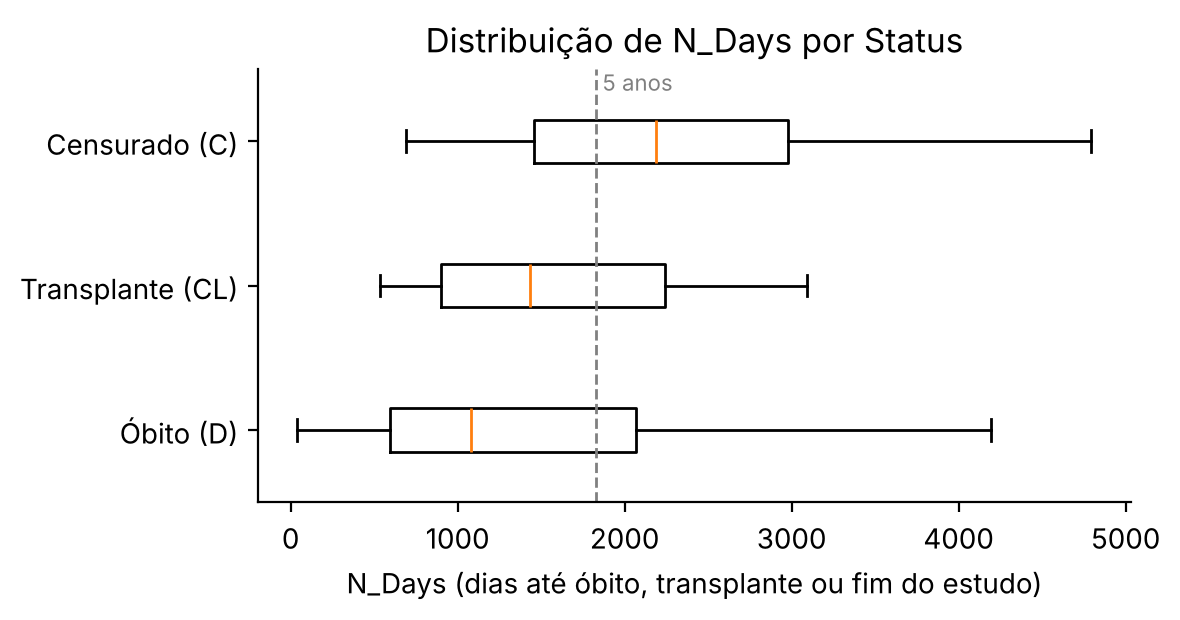
\includegraphics[width=0.72\linewidth]{figuras/n_days_por_status.png}
\caption{Distribuição do tempo de seguimento (\texttt{N\_Days}) por desfecho; a linha tracejada marca o horizonte de cinco anos.}
\label{fig:ndays}
\par\vspace{3pt}{\footnotesize\color{cinzasec}Fonte: elaboração própria a partir de \citeonline{uci878}; 418 pacientes.}
\end{figure}

\subsection{Estratégia de validação e prevenção de vazamento}
A avaliação principal usa validação cruzada estratificada repetida, com 5 repetições de 5 partições (25 avaliações) e as mesmas divisões para todos os modelos. O ajuste de hiperparâmetros é aninhado \cite{varma2006bias}: em cada partição externa, uma busca aleatória com 3 partições internas, critério AUROC e 12 configurações sorteadas usa só o treino. A predição fora da partição de cada paciente é a média das 5 repetições. A variável \texttt{N\_Days} nunca é entrada, porque só é conhecida depois do desfecho.

Duas análises complementares testam a generalização e o vazamento. Na validação quase externa, os modelos são desenvolvidos nos 244 pacientes rotulados do ensaio randomizado (85 óbitos, 34,8\%) e testados nos 68 rotulados não randomizados (30 óbitos, 44,1\%). Nesse teste, as variáveis exclusivas do ensaio estão ausentes e são imputadas ou tratadas nativamente. No braço de controle de vazamento, o enquadramento da competição do Kaggle é reproduzido: classificação de \texttt{Status} em três classes nos 418 pacientes, com XGBoost e as 17 variáveis, com e sem \texttt{N\_Days} como entrada, na mesma validação 5 x 5.

\subsection{Algoritmos e ajuste de hiperparâmetros}
Seja $\mathbf{x}_i$ o vetor de variáveis de linha de base do paciente $i$ e $y_i \in \{0,1\}$ o indicador de óbito em até cinco anos. Cada modelo estima $\hat{\pi}(\mathbf{x}) = \hat{P}(y=1 \mid \mathbf{x})$.

\textbf{Escore de Mayo (referência histórica).} O modelo final de \citeonline{dickson1989prognosis}, estimado com os 418 pacientes, define o escore
\begin{equation}
\begin{aligned}
R ={}& 0{,}039\,\text{idade} + 0{,}871\ln(\text{bilirrubina}) - 2{,}53\ln(\text{albumina})\\
&+ 2{,}38\ln(\text{protrombina}) + 0{,}859\,\text{edema},
\end{aligned}
\label{eq:mayo}
\end{equation}
e a implementação reproduz os dois exemplos resolvidos do artigo original ($R = 3{,}12$ e $R = 8{,}39$). A probabilidade original de óbito em cinco anos é $\hat{\pi} = 1 - 0{,}774^{\exp(R - 5{,}07)}$, em que 0,774 é a sobrevida basal em cinco anos e 5,07 é a média de $R$ na coorte. Como esses coeficientes foram estimados nos mesmos pacientes usados aqui, inclusive nos de teste, o escore publicado entra apenas como referência histórica, em duas versões: a probabilidade original e uma versão recalibrada no treino, $\hat{\pi} = \sigma(a + bR)$, com $\sigma(z) = 1/(1+e^{-z})$. Na validação quase externa entra também o modelo inicial de \citeonline{dickson1989prognosis}, estimado só com os 312 pacientes randomizados e, portanto, sem contato com o teste.

\textbf{Regressão logística com as 5 variáveis de Mayo (referência principal).} O modelo $\hat{\pi}(\mathbf{x}) = \sigma(\beta_0 + \boldsymbol{\beta}^\top \tilde{\mathbf{x}})$, com as variáveis transformadas e padronizadas $\tilde{\mathbf{x}}$, é estimado por máxima verossimilhança em cada partição. É o Escore de Mayo reestimado, livre do vazamento dos coeficientes publicados.

\textbf{Regressão logística com 17 variáveis.} Penalização \textit{elastic net} \cite{zou2005elasticnet}, que minimiza a perda logística mais $\frac{1}{C}\big(\alpha\|\boldsymbol{\beta}\|_1 + \frac{1-\alpha}{2}\|\boldsymbol{\beta}\|_2^2\big)$, com $C \in \{0{,}01;\,0{,}03;\,0{,}1;\,0{,}3;\,1;\,3\}$ e $\alpha \in \{0;\,0{,}5;\,1\}$.

\textbf{\textit{Random forest}.} Média de 300 árvores de classificação, cada uma treinada numa amostra \textit{bootstrap} e escolhendo cada divisão entre um subconjunto aleatório de variáveis \cite{breiman2001random}. Grade: tamanho mínimo da folha em $\{3, 5, 10, 20\}$, variáveis por divisão em $\{\sqrt{p}, 0{,}5p, p\}$ e profundidade em $\{$livre$, 4, 6\}$.

\textbf{XGBoost.} Modelo aditivo de árvores ajustadas por gradiente com aproximação de segunda ordem e regularização \cite{chen2016xgboost}. Grade: número de árvores em $\{100, 200, 400\}$, taxa de aprendizado em $\{0{,}02;\,0{,}05;\,0{,}1\}$, profundidade em $\{1, 2, 3\}$, peso mínimo por folha em $\{1, 5\}$ e regularização L2 em $\{1, 5\}$.

Nas tabelas, RL designa a regressão logística e RF, o \textit{random forest}. As grades foram definidas antes de qualquer resultado e não foram alteradas depois. Todos os modelos com busca usam o mesmo orçamento de 12 configurações. Na análise de sensibilidade, \textit{random forest} e XGBoost com 17 variáveis recebem exatamente o pré-processamento da regressão com 17 variáveis (logaritmo, imputação iterativa e padronização). Como árvores são invariantes a transformações monotônicas, a diferença restante em relação à regressão é o algoritmo com seus hiperparâmetros.

\subsection{Métricas de avaliação}\label{subsec:metricas}
A métrica principal é a área sob a curva ROC (AUROC), a probabilidade de o modelo atribuir risco maior a um paciente que morreu do que a um que sobreviveu \cite{fawcett2006roc}. Complementam a discriminação a precisão média (AP, soma da precisão ponderada pelos incrementos de revocação) e, num limiar de 0,5, precisão, sensibilidade (revocação), especificidade e F1. A sensibilidade é
\begin{equation}
\operatorname{Sensibilidade}=\frac{VP}{VP+FN},
\label{eq:sensibilidade}
\end{equation}
em que $VP$ é o número de verdadeiros positivos e $FN$ o de falsos negativos. A exatidão das probabilidades é medida pelo escore de Brier, $\frac{1}{n}\sum_i(\hat{\pi}_i - y_i)^2$, e pela calibração \cite{vancalster2019calibration}. A calibração no geral (CITL) é o intercepto $a$ em $\operatorname{logit} P(y=1) = a + \operatorname{logit}(\hat{\pi})$, ajustado com o logito da predição como \textit{offset}; o ideal é 0, valores positivos indicam subestimação do risco e negativos, superestimação. A inclinação de calibração é o coeficiente $b$ em $\operatorname{logit} P(y=1) = a + b\,\operatorname{logit}(\hat{\pi})$; o ideal é 1, e valores acima de 1 indicam probabilidades comprimidas demais.

O valor incremental é a diferença de AUROC ($\Delta$AUROC) entre cada modelo e a referência, calculada sobre as predições fora da partição. Os intervalos de confiança vêm de 2.000 reamostragens \textit{bootstrap} pareadas de pacientes. Para as cinco comparações principais, além do IC 95\%, calcula-se um IC simultâneo de Bonferroni de 99\% (nível $1 - 0{,}05/5$), e só se afirma ``maior'' ou ``menor'' quando ele exclui zero. Esses intervalos são condicionais às predições já obtidas, isto é, não incorporam a variação de refazer o treino e a busca de hiperparâmetros, e por isso são exploratórios. Como nenhuma margem de equivalência foi definida a priori, ``sem evidência de diferença'' não significa equivalência. A variação do treino aparece na dispersão da diferença de AUROC entre as 25 partições.

\subsection{Reprodutibilidade e aspectos éticos}
O experimento foi executado em Python 3.13 com scikit-learn 1.9.1 e XGBoost 3.4.1, com versões fixadas, semente 2026 em todos os componentes aleatórios e verificação SHA-256 da cópia dos dados. Os hiperparâmetros escolhidos em cada partição foram salvos, e nenhum aviso de convergência ocorreu. Duas execuções completas do notebook, guardadas em commits distintos do repositório, produziram os mesmos resultados, com diferença absoluta máxima de $1{,}6 \times 10^{-13}$; o script de comparação e sua saída estão em \texttt{auditoria/}. Código, notebook, dados e resultados estão em \url{https://github.com/claytonchagas/ml4health}, e o código e as conclusões passaram por duas rodadas de auditoria independente por outro agente de IA. Os dados são públicos, anonimizados e licenciados para reúso, o que dispensa aprovação ética para esta análise secundária.

% ================================= RESULTADOS ================================
\section{Resultados}\label{sec:resultados}

\subsection{Caracterização do conjunto analisado}
A análise principal usa os 312 pacientes rotulados: 197 vivos aos cinco anos e 115 óbitos (36,9\%). Todos os modelos foram avaliados nesses 312 pacientes, com imputação ou tratamento nativo dos ausentes. A Tabela~\ref{tab:caracterizacao} compara os dois grupos. Os pacientes que morreram eram mais velhos e tinham, na linha de base, bilirrubina muito mais alta, albumina mais baixa, tempo de protrombina mais longo, edema e ascite mais frequentes e estágio histológico mais avançado, o mesmo padrão que deu origem às variáveis do Escore de Mayo.

\begin{table}[htbp]
\centering
\caption{Características da linha de base por desfecho em cinco anos (312 pacientes rotulados).}
\label{tab:caracterizacao}
\small
\renewcommand{\arraystretch}{1.12}
\begin{adjustbox}{max width=\linewidth}
\begin{tabular}{@{}lccc@{}}
\toprule
\textbf{Variável} & \textbf{Vivos (n = 197)} & \textbf{Óbitos (n = 115)} & \textbf{Ausentes} \\
\midrule
Idade (anos) & 49,8 (42,6--56,0) & 53,9 (46,7--61,8) & 0 \\
Sexo masculino (\%) & 8,1 & 15,7 & 0 \\
Bilirrubina (mg/dL) & 0,90 (0,60--1,60) & 4,40 (2,30--10,15) & 0 \\
Albumina (g/dL) & 3,67 (3,48--3,94) & 3,26 (3,01--3,52) & 0 \\
Tempo de protrombina (s) & 10,45 (10,00--11,00) & 11,10 (10,53--11,97) & 2 \\
Edema presente (\%) & 7,6 & 34,8 & 0 \\
Ascite (\%)\textsuperscript{a} & 1,9 & 23,5 & 68 \\
Plaquetas ($10^3$/mm$^3$) & 266,5 (202,5--336,3) & 214 (156--292) & 11 \\
Estágio histológico & 3 (2--3) & 4 (3--4) & 6 \\
\bottomrule
\end{tabular}
\end{adjustbox}
\par\vspace{3pt}{\footnotesize\color{cinzasec}Fonte: elaboração própria. Valores numéricos em mediana (intervalo interquartil). \textsuperscript{a}Entre os pacientes com o dado; ausente nos 68 rotulados fora do ensaio.}
\end{table}

\subsection{Comparação do desempenho dos modelos}
A Tabela~\ref{tab:resultados} apresenta o desempenho na validação cruzada 5 x 5. A referência principal, a regressão logística com as 5 variáveis de Mayo, teve AUROC média de 0,906 e estimativas de calibração próximas das ideais (CITL de $-$0,01 e inclinação de 1,04). A maior AUROC nominal foi a da regressão penalizada com 17 variáveis (0,915). \textit{Random forest} e XGBoost ficaram entre 0,891 e 0,903 nas configurações principais. A dispersão entre partições (desvio de 0,035 a 0,051) é maior do que qualquer diferença entre modelos.

\begin{table}[htbp]
\centering
\caption{Desempenho na validação cruzada 5 x 5 (média $\pm$ desvio entre as 25 partições; 312 pacientes).}
\label{tab:resultados}
\footnotesize
\renewcommand{\arraystretch}{1.16}
\setlength{\tabcolsep}{4pt}
\begin{adjustbox}{max width=\linewidth}
\begin{tabular}{@{}lccccc@{}}
\toprule
\textbf{Modelo} & \textbf{AUROC} & \textbf{AP} & \textbf{Brier} & \textbf{CITL} & \textbf{Inclinação} \\
\midrule
\textit{Mayo 1989, prob. original}\textsuperscript{a} & 0,910 $\pm$ 0,040 & 0,879 $\pm$ 0,054 & 0,121 $\pm$ 0,023 & 0,33 $\pm$ 0,18 & 1,56 $\pm$ 0,44 \\
\textit{Mayo 1989, recalibrado}\textsuperscript{a} & 0,910 $\pm$ 0,040 & 0,879 $\pm$ 0,054 & 0,112 $\pm$ 0,028 & 0,00 $\pm$ 0,31 & 1,10 $\pm$ 0,33 \\
\textbf{RL, 5 var. (referência)} & \textbf{0,906 $\pm$ 0,044} & \textbf{0,871 $\pm$ 0,061} & \textbf{0,115 $\pm$ 0,032} & \textbf{$-$0,01 $\pm$ 0,33} & \textbf{1,04 $\pm$ 0,36} \\
RL \textit{elastic net}, 17 var. & 0,915 $\pm$ 0,035 & 0,880 $\pm$ 0,051 & 0,121 $\pm$ 0,024 & 0,00 $\pm$ 0,25 & 1,74 $\pm$ 0,91 \\
RF, 5 var. & 0,893 $\pm$ 0,047 & 0,852 $\pm$ 0,066 & 0,130 $\pm$ 0,030 & 0,01 $\pm$ 0,27 & 1,27 $\pm$ 0,60 \\
RF, 17 var. & 0,903 $\pm$ 0,044 & 0,862 $\pm$ 0,069 & 0,124 $\pm$ 0,026 & 0,02 $\pm$ 0,21 & 1,57 $\pm$ 0,58 \\
XGBoost, 5 var. & 0,891 $\pm$ 0,051 & 0,852 $\pm$ 0,072 & 0,126 $\pm$ 0,033 & 0,04 $\pm$ 0,26 & 1,09 $\pm$ 0,34 \\
XGBoost, 17 var. & 0,895 $\pm$ 0,042 & 0,854 $\pm$ 0,064 & 0,126 $\pm$ 0,028 & 0,04 $\pm$ 0,26 & 1,15 $\pm$ 0,41 \\
RF, 17 var., pré-proc. da RL\textsuperscript{b} & 0,907 $\pm$ 0,042 & 0,868 $\pm$ 0,063 & 0,122 $\pm$ 0,024 & 0,00 $\pm$ 0,20 & 1,52 $\pm$ 0,60 \\
XGBoost, 17 var., pré-proc. da RL\textsuperscript{b} & 0,899 $\pm$ 0,039 & 0,855 $\pm$ 0,053 & 0,126 $\pm$ 0,027 & 0,07 $\pm$ 0,33 & 1,04 $\pm$ 0,46 \\
\bottomrule
\end{tabular}
\end{adjustbox}
\par\vspace{3pt}{\footnotesize\color{cinzasec}Fonte: elaboração própria. \textsuperscript{a}Referência histórica: coeficientes estimados com os mesmos pacientes, inclusive os de teste. \textsuperscript{b}Análise de sensibilidade com o pré-processamento da regressão logística (RL).}
\end{table}

A Tabela~\ref{tab:incremental} mostra o valor incremental sobre a referência. Em nenhuma das cinco comparações o IC de Bonferroni excluiu zero. A regressão penalizada com 17 variáveis teve a maior diferença nominal (+0,009) e superou a referência em 60\% das partições. Os modelos de AM ficaram nominalmente abaixo da referência ($-$0,013 a 0,000) e a superaram em apenas 20\% a 40\% das partições. O XGBoost com 5 variáveis teve IC 95\% inteiramente negativo, mas o IC de Bonferroni incluiu zero.

\begin{table}[htbp]
\centering
\caption{Valor incremental em AUROC sobre a regressão logística com as 5 variáveis de Mayo.}
\label{tab:incremental}
\footnotesize
\renewcommand{\arraystretch}{1.16}
\setlength{\tabcolsep}{4pt}
\begin{adjustbox}{max width=\linewidth}
\begin{tabular}{@{}lccccc@{}}
\toprule
\textbf{Modelo} & \textbf{$\Delta$AUROC} & \textbf{IC 95\%} & \textbf{IC 99\% (Bonferroni)} & \textbf{$\Delta$ por partição} & \textbf{Partições com ganho} \\
\midrule
RL \textit{elastic net}, 17 var. & +0,009 & [$-$0,010; 0,030] & [$-$0,017; 0,035] & +0,009 $\pm$ 0,027 & 60\% \\
RF, 5 var. & $-$0,013 & [$-$0,029; 0,003] & [$-$0,035; 0,009] & $-$0,013 $\pm$ 0,019 & 24\% \\
RF, 17 var. & 0,000 & [$-$0,018; 0,016] & [$-$0,022; 0,024] & $-$0,003 $\pm$ 0,018 & 40\% \\
XGBoost, 5 var. & $-$0,013 & [$-$0,027; $-$0,001] & [$-$0,031; 0,003] & $-$0,016 $\pm$ 0,019 & 20\% \\
XGBoost, 17 var. & $-$0,006 & [$-$0,025; 0,012] & [$-$0,030; 0,017] & $-$0,011 $\pm$ 0,019 & 24\% \\
\bottomrule
\end{tabular}
\end{adjustbox}
\par\vspace{3pt}{\footnotesize\color{cinzasec}Fonte: elaboração própria. Intervalos por \textit{bootstrap} pareado de pacientes (2.000 reamostragens), condicionais às predições fora da partição e, por isso, exploratórios. Leitura em todas as linhas: sem evidência de diferença.}
\end{table}

No desenho 2 x 2, as 12 variáveis extras acrescentaram cerca de 0,01 de AUROC nominal em cada família (regressão: 0,906 para 0,915; \textit{random forest}: 0,893 para 0,903; XGBoost: 0,891 para 0,895), sem contraste inferencial próprio. Na leitura vertical, a regressão teve a maior AUROC nominal nas duas colunas. Com o pré-processamento da regressão, \textit{random forest} e XGBoost com 17 variáveis também não mostraram ganho sobre a regressão penalizada ($-$0,006, IC de Bonferroni de 97,5\% [$-$0,023; 0,011]; e $-$0,013 [$-$0,030; 0,004]). Nominalmente, esse pré-processamento elevou a AUROC das árvores (de 0,903 para 0,907 e de 0,895 para 0,899), mas esse efeito não foi testado diretamente.

A Figura~\ref{fig:roc} mostra a distribuição das AUROCs por partição, as curvas ROC sobre as predições fora da partição e a calibração por decis de risco. As curvas ROC praticamente se sobrepõem. Na calibração, a probabilidade original do Escore de Mayo fica acima da diagonal em quase toda a faixa, ou seja, subestima o risco observado, enquanto os demais modelos ficam próximos da diagonal, com oscilações entre decis; com cerca de 31 pacientes por decil, a figura é descritiva e não traz bandas de incerteza.

\begin{figure}[htbp]
\centering
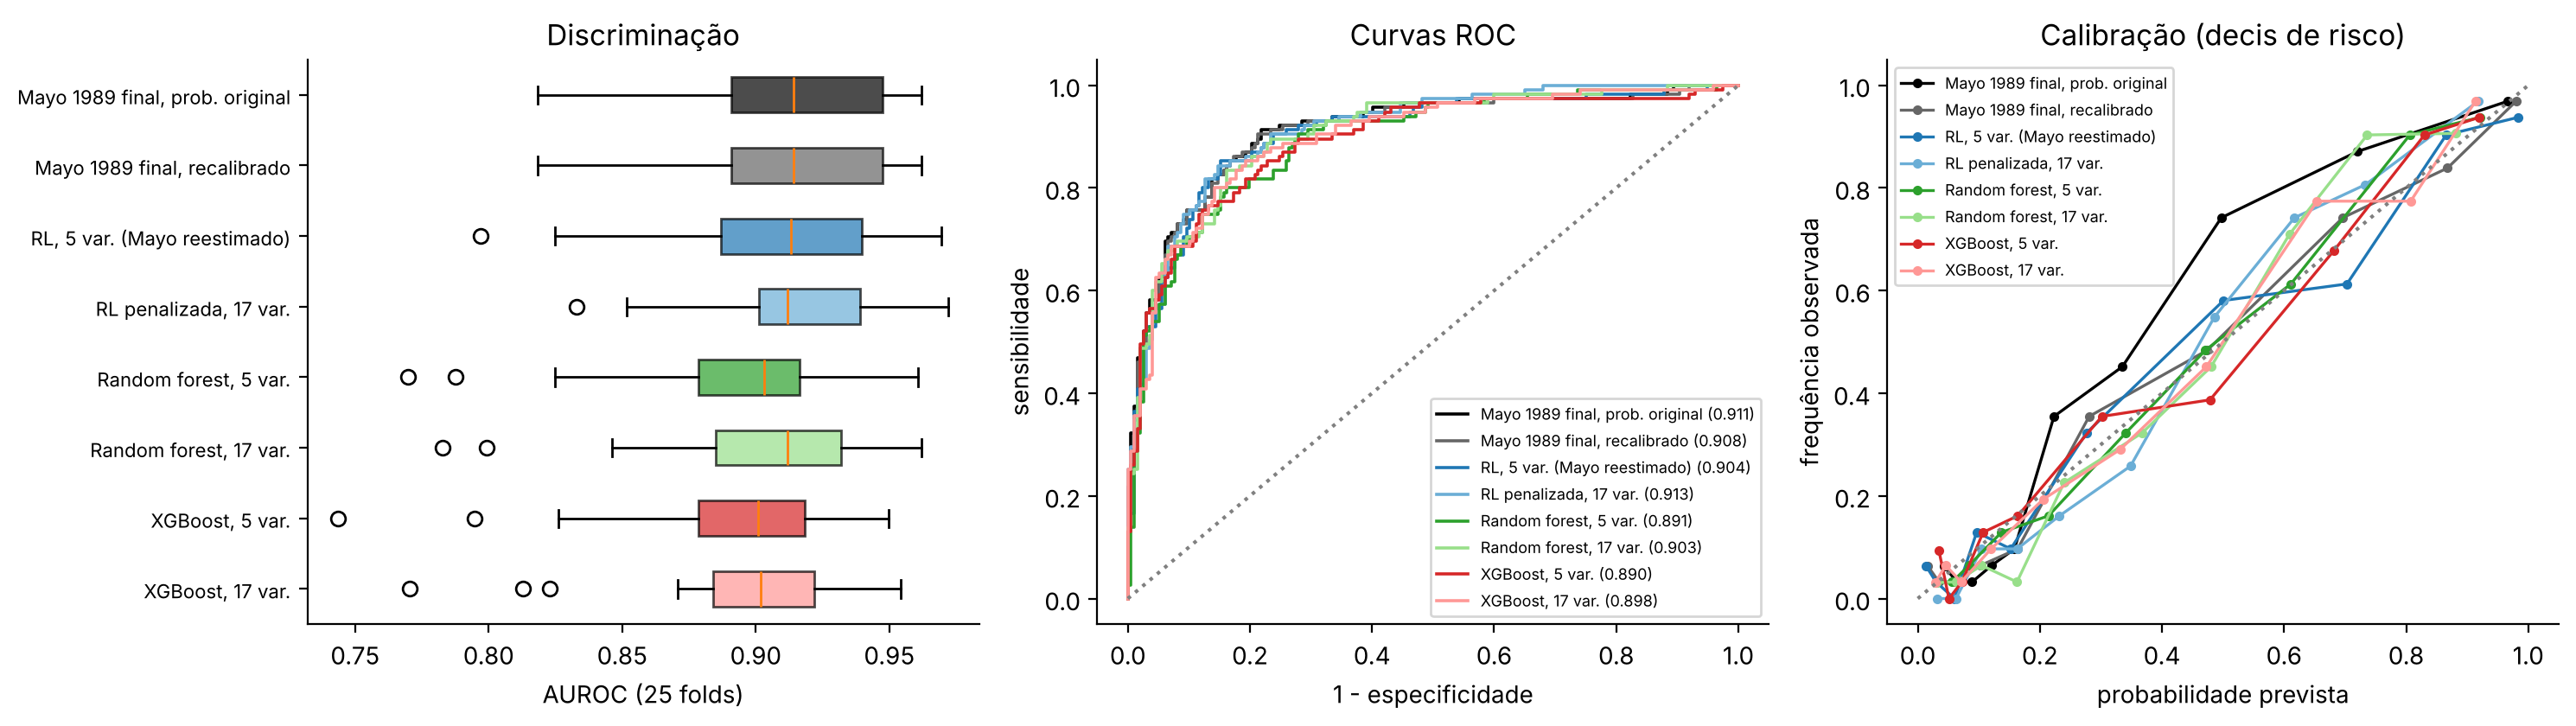
\includegraphics[width=\linewidth]{figuras/discriminacao_roc_calibracao.png}
\caption{AUROC nas 25 partições (esquerda), curvas ROC sobre as predições fora da partição (centro) e calibração por decis de risco (direita).}
\label{fig:roc}
\par\vspace{3pt}{\footnotesize\color{cinzasec}Fonte: elaboração própria; 312 pacientes. A AUROC da legenda é calculada sobre as predições médias e difere ligeiramente da média por partição da Tabela~\ref{tab:resultados}.}
\end{figure}

\subsection{Análise de erros e resultados complementares}
\textbf{Erros no limiar de 0,5.} A Tabela~\ref{tab:limiar} traduz as probabilidades em decisões, usando o limiar de 0,5 sobre as predições fora da partição. O limiar é ilustrativo, pois nenhum limiar clínico foi definido para esta população. A referência identificou 89 dos 115 óbitos (sensibilidade de 0,774), com 23 falsos positivos entre 197 sobreviventes. Os modelos de AM das configurações principais deixaram de identificar de 32 a 34 óbitos, contra 26 da referência. A probabilidade original do Escore de Mayo teve a maior precisão (0,873), mas a menor sensibilidade (0,600), consequência direta da subestimação do risco: com probabilidades baixas demais, menos pacientes ultrapassam o limiar.

\begin{table}[htbp]
\centering
\caption{Medidas de classificação no limiar de 0,5 (predições fora da partição; 115 óbitos e 197 sobreviventes).}
\label{tab:limiar}
\small
\renewcommand{\arraystretch}{1.14}
\begin{adjustbox}{max width=\linewidth}
\begin{tabular}{@{}lccccc@{}}
\toprule
\textbf{Modelo} & \textbf{Precisão} & \textbf{Sensibilidade} & \textbf{Especificidade} & \textbf{F1} & \textbf{Óbitos não detectados} \\
\midrule
\textit{Mayo 1989, prob. original} & 0,873 & 0,600 & 0,949 & 0,711 & 46 \\
\textit{Mayo 1989, recalibrado} & 0,821 & 0,757 & 0,904 & 0,787 & 28 \\
\textbf{RL, 5 var.} & \textbf{0,795} & \textbf{0,774} & \textbf{0,883} & \textbf{0,784} & \textbf{26} \\
RL \textit{elastic net}, 17 var. & 0,819 & 0,748 & 0,904 & 0,782 & 29 \\
RF, 5 var. & 0,794 & 0,704 & 0,893 & 0,747 & 34 \\
RF, 17 var. & 0,781 & 0,713 & 0,883 & 0,745 & 33 \\
XGBoost, 5 var. & 0,786 & 0,704 & 0,888 & 0,743 & 34 \\
XGBoost, 17 var. & 0,790 & 0,722 & 0,888 & 0,755 & 32 \\
\bottomrule
\end{tabular}
\end{adjustbox}
\par\vspace{3pt}{\footnotesize\color{cinzasec}Fonte: elaboração própria. Sensibilidade equivale à revocação (\textit{recall}). Análise descritiva, sem intervalos de confiança.}
\end{table}

\textbf{Referência histórica.} Contra a probabilidade original do Escore de Mayo publicado, a regressão reestimada com 5 variáveis ficou em $-$0,007 (IC de Bonferroni [$-$0,018; 0,003]), e \textit{random forest} e XGBoost com 5 variáveis ficaram abaixo ($-$0,021 cada, com IC de Bonferroni que exclui zero). Essa comparação favorece o escore, cujos coeficientes foram estimados com os pacientes de teste, e por isso não sustenta inferências sobre o valor do escore em pacientes novos.

\textbf{Validação quase externa.} A Tabela~\ref{tab:quase} apresenta o desempenho no teste com os 68 pacientes não randomizados. O comparador histórico válido é o modelo inicial de Dickson, estimado sem esses pacientes (AUROC de 0,865). A mortalidade no teste (44,1\%) foi maior que no treino (34,8\%), e quase todos os modelos subestimaram o risco (CITL entre +0,30 e +0,85). A exceção foi o XGBoost com 17 variáveis, que perdeu discriminação (0,845) e superestimou o risco (CITL de $-$0,81). Com o pré-processamento da regressão, o mesmo algoritmo chegou a 0,888. Com 68 pacientes e 30 óbitos, nenhum intervalo de confiança foi calculado, e diferenças de alguns centésimos não devem ser interpretadas. A análise é descritiva e serve para sinalizar quedas grandes de discriminação e desvios de calibração.

\begin{table}[htbp]
\centering
\caption{Validação quase externa: treino nos 244 pacientes do ensaio, teste nos 68 não randomizados (30 óbitos).}
\label{tab:quase}
\small
\renewcommand{\arraystretch}{1.14}
\begin{adjustbox}{max width=\linewidth}
\begin{tabular}{@{}lccccc@{}}
\toprule
\textbf{Modelo} & \textbf{AUROC} & \textbf{AP} & \textbf{Brier} & \textbf{CITL} & \textbf{Inclinação} \\
\midrule
Mayo 1989 inicial (n = 312), recalibrado & 0,865 & 0,847 & 0,155 & 0,33 & 0,83 \\
RL, 5 var. & 0,878 & 0,844 & 0,144 & 0,30 & 0,88 \\
RL \textit{elastic net}, 17 var. & 0,874 & 0,859 & 0,172 & 0,46 & 2,27 \\
RF, 5 var. & 0,882 & 0,876 & 0,145 & 0,41 & 1,15 \\
RF, 17 var. & 0,896 & 0,876 & 0,145 & 0,30 & 1,49 \\
XGBoost, 5 var. & 0,879 & 0,870 & 0,145 & 0,38 & 0,99 \\
XGBoost, 17 var. & 0,845 & 0,842 & 0,179 & $-$0,81 & 1,00 \\
RF, 17 var., pré-proc. da RL & 0,897 & 0,882 & 0,149 & 0,79 & 0,98 \\
XGBoost, 17 var., pré-proc. da RL & 0,888 & 0,878 & 0,150 & 0,85 & 0,66 \\
\bottomrule
\end{tabular}
\end{adjustbox}
\par\vspace{3pt}{\footnotesize\color{cinzasec}Fonte: elaboração própria. Os coeficientes finais de Mayo foram estimados com os 418 pacientes, inclusive os 68 do teste, e foram omitidos desta tabela (estão no repositório).}
\end{table}

\textbf{Vazamento por \texttt{N\_Days}.} No enquadramento da competição do Kaggle (três classes, 418 pacientes, XGBoost com 17 variáveis), incluir \texttt{N\_Days} como entrada reduziu o \textit{log loss} de 0,753 $\pm$ 0,089 para 0,645 $\pm$ 0,086, elevou a AUROC macro de 0,788 $\pm$ 0,043 para 0,822 $\pm$ 0,045 e a acurácia de 0,721 $\pm$ 0,037 para 0,763 $\pm$ 0,032 (Figura~\ref{fig:vazamento}). O ganho vem de uma informação que não existe no momento da predição.

\begin{figure}[htbp]
\centering
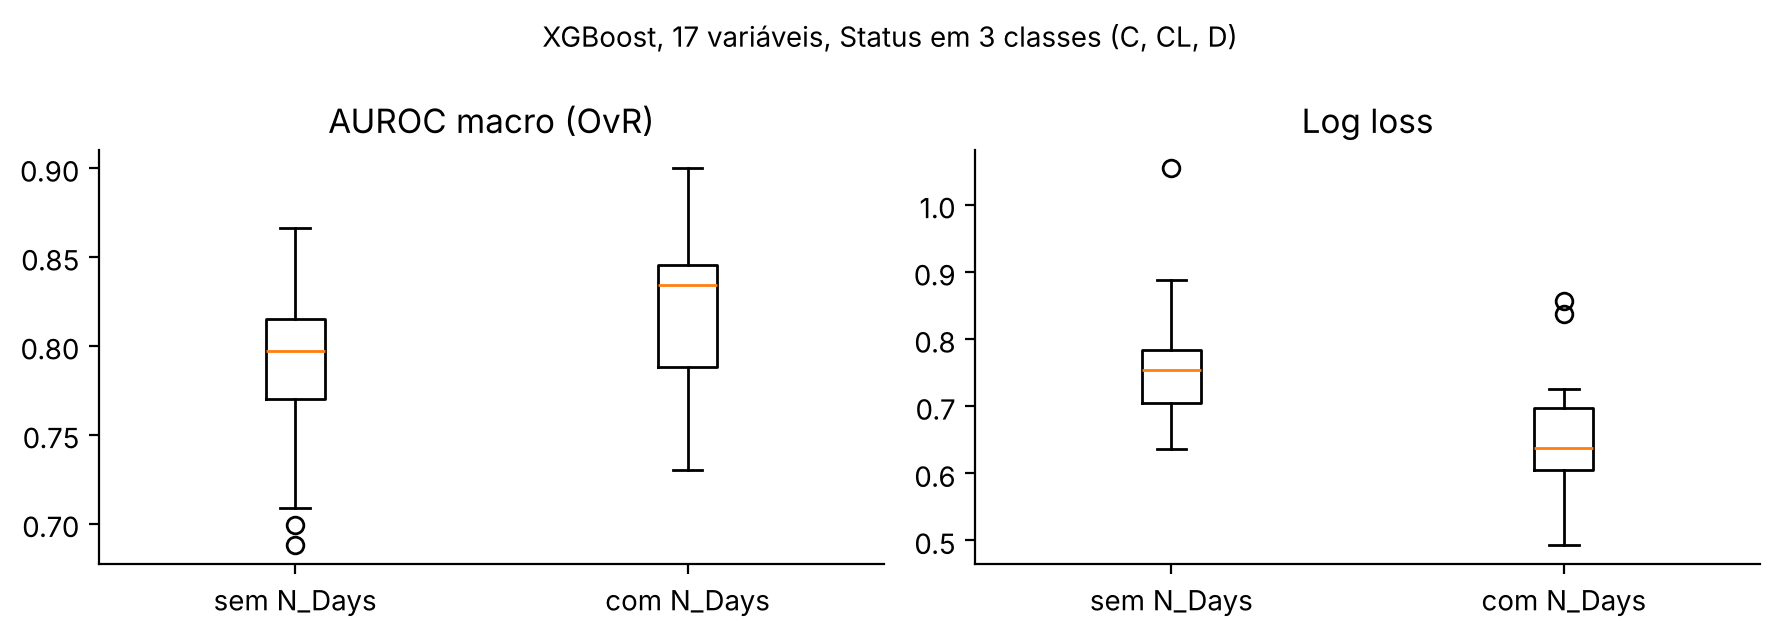
\includegraphics[width=0.78\linewidth]{figuras/vazamento_n_days.png}
\caption{Efeito de usar \texttt{N\_Days} como entrada no enquadramento de três classes (25 partições).}
\label{fig:vazamento}
\par\vspace{3pt}{\footnotesize\color{cinzasec}Fonte: elaboração própria; 418 pacientes.}
\end{figure}

% ================================= DISCUSSAO =================================
\section{Discussão}\label{sec:discussao}

O resultado principal é negativo e consistente: nenhum modelo de AM demonstrou ganho de discriminação sobre uma regressão logística com as cinco variáveis do Escore de Mayo, e as diferenças em relação à referência, entre $-$0,013 e +0,009 de AUROC, são menores que a variação entre partições (desvios de 0,035 a 0,051). Esse resultado responde à pergunta do título num sentido prático. Com as mesmas cinco variáveis, o AM não exige dados extras, mas troca uma fórmula transparente por um modelo opaco sem ganho demonstrado. Passar para 17 variáveis acrescenta, a qualquer família, o custo de coleta e a menor elegibilidade sem imputação (de 310 para 210 pacientes com dados completos), também sem ganho demonstrado. O fato de a regressão penalizada com 17 variáveis ter tido a maior AUROC nominal indica que, nestes dados, as árvores não extraíram das variáveis extras mais informação do que um modelo linear; o desenho não testa se as duas famílias as aproveitam igualmente.

O achado está alinhado com a revisão de \citeonline{christodoulou2019systematic}, que não encontrou vantagem do AM sobre a regressão logística nas comparações com baixo risco de viés. Há uma explicação plausível para isso neste problema: com 312 pacientes e 115 eventos, o espaço para aprender interações e não linearidades que um modelo linear em escala logarítmica não capture é pequeno, e o próprio Escore de Mayo já incorpora as transformações que tornam a relação aproximadamente linear. Essa explicação, no entanto, é uma hipótese; o desenho não a testa. Os números relatados nos trabalhos que seguem o enquadramento do Kaggle, com acurácias próximas de 90\% \cite{shakir2025cirrhosis,tu2025cirrhosis}, não são comparáveis com os deste estudo, porque usam outro desfecho (três classes ou óbito sem horizonte), outros dados (sintéticos) e outro protocolo de avaliação.

A calibração diferenciou os modelos mais do que a discriminação. A probabilidade original do Escore de Mayo teve AUROC média de 0,910, obtida com coeficientes estimados nos próprios pacientes de teste, mas subestimou o risco (CITL de +0,33), o que se traduziu em 46 óbitos não detectados no limiar de 0,5, contra 26 da regressão reestimada. Uma explicação possível, não testada, é a definição do rótulo: ao excluir os pacientes censurados antes de cinco anos, a amostra rotulada fica com mais óbitos do que a coorte de onde a sobrevida basal foi estimada. Recalibrado no treino, o escore teve estimativas de calibração próximas das ideais (CITL de 0,00 e inclinação de 1,10). Entre os modelos treinados, a regressão penalizada e o \textit{random forest} com 17 variáveis produziram probabilidades comprimidas demais (inclinações de 1,74 e 1,57), um problema que a AUROC não revela e que afetaria o uso clínico das probabilidades \cite{vancalster2019calibration}. Na validação quase externa, a regressão penalizada escolheu uma penalização forte, e sua inclinação de calibração chegou a 2,27.

O braço de controle mostra o tamanho do problema do vazamento neste conjunto. Incluir o tempo de seguimento como entrada reduziu o \textit{log loss} em 14\% e elevou a AUROC macro em 0,034, um ganho maior do que qualquer diferença entre algoritmos observada na análise principal. Um estudo que compare algoritmos nesse enquadramento pode, portanto, atribuir ao algoritmo um desempenho que vem da informação vazada \cite{kapoor2023leakage}.

O estudo tem limitações importantes. Os dados vêm de um único centro, nas décadas de 1970 e 1980, antes do uso do ácido ursodesoxicólico, e não representam os pacientes atuais. Não houve coorte externa verdadeira: a validação quase externa usa pacientes do mesmo centro e período, com apenas 68 pacientes, e os coeficientes publicados de Mayo foram estimados nesses dados, o que limita o escore publicado ao papel de referência histórica. A classificação com horizonte fixo exclui 106 pacientes censurados ou transplantados antes de cinco anos; a análise de sobrevivência com riscos competitivos é a extensão natural. Os intervalos de confiança são condicionais às predições fora da partição e não incorporam a variação de refazer o treino, o que os torna exploratórios, e não houve teste de equivalência. Por fim, o orçamento de busca de hiperparâmetros foi modesto (12 configurações), e a conclusão vale para os algoritmos, as grades e o orçamento avaliados. Estes resultados descrevem desempenho retrospectivo e não constituem evidência de utilidade clínica.

% ================================= CONCLUSAO =================================
\section{Conclusão}\label{sec:conclusao}

Este estudo mediu o valor incremental de \textit{random forest} e XGBoost sobre uma regressão logística com as cinco variáveis do Escore de Mayo na predição de óbito em até cinco anos na cirrose biliar primária. Num desenho 2 x 2, com as mesmas partições e o mesmo orçamento de ajuste para todos os modelos, nenhum modelo de AM demonstrou ganho, nem com as 5 variáveis nem com as 17, e a referência teve AUROC nominalmente próxima da dos demais modelos, sem diferença demonstrada, e estimativas de calibração próximas das ideais. Neste estudo de caso, um modelo de regressão com cinco variáveis de rotina vale mais a pena: o ganho do AM não foi demonstrado, e seus custos, em transparência e, com 17 variáveis, em coleta de dados, são concretos. O braço de controle mostrou ainda que o enquadramento da competição do Kaggle, com o tempo de seguimento como entrada, infla o desempenho com uma informação indisponível no momento da predição.

A continuidade natural é tratar o problema como análise de sobrevivência, comparando o modelo de Cox com \textit{random survival forests} sem excluir os pacientes censurados, e repetir a comparação em coortes atuais de pacientes tratados com ácido ursodesoxicólico, em que escores como o GLOBE e o UK-PBC são as referências clínicas. Em ambos os casos, a pergunta deve continuar sendo a do valor incremental: quanto o novo modelo acrescenta ao que a clínica já usa, e a que custo.


% ================================ BIBLIOGRAFIA ===============================
% Bibliografia em BibTeX; abntex2cite [alf] configura estilo autor-data ABNT.
\bibliography{referencias}
\end{document}
